\documentclass[11pt,a4paper]{article}

%%%%%%%%%%%%%%%%%%%%%%%%%%%%%%%%%%
% Encoding and language
\usepackage[utf8]{inputenc}
\usepackage[T1]{fontenc}
\usepackage[english]{babel}
\selectlanguage{English}

%%%%%%%%%%%%%%%%%%%%%%%%%%%%%%%%%%
% General packages
\usepackage{verbatim}
\usepackage[all]{xy}
\usepackage{float}
\usepackage{amsmath}
\usepackage{array}
\usepackage{listings}
\usepackage{xcolor}
\usepackage{setspace}
\usepackage{booktabs}
\usepackage{graphicx}
\usepackage{url}
\usepackage{lmodern}
\interfootnotelinepenalty=10000

%%%%%%%%%%%%%%%%%%%%%%%%%%%%%%%%%%
% Page layout
\usepackage{geometry}
\geometry{margin=2.5cm}

%%%%%%%%%%%%%%%%%%%%%%%%%%%%%%%%%%
% Hyperlinks
\usepackage[
    colorlinks=true,
    urlcolor=blue!50!black,
    linkcolor=black,
    citecolor=black
]{hyperref}

%%%%%%%%%%%%%%%%%%%%%%%%%%%%%%%%%%
% Bibliography
\usepackage[round]{natbib}

%%%%%%%%%%%%%%%%%%%%%%%%%%%%%%%%%%
% Fancy headers (ALL pages incl. title page)
\usepackage{fancyhdr}
\pagestyle{fancy}

\fancyhf{} % clear header/footer

\fancyhead[L]{zpn710, fps618, kvb125, xnc401 - everyone contributed equally}
\fancyhead[R]{February 2026}
\fancyfoot[C]{\thepage}

\renewcommand{\headrulewidth}{0.4pt}
\renewcommand{\footrulewidth}{0pt}

% IMPORTANT: make 'plain' style match 'fancy'
\fancypagestyle{plain}{
    \fancyhf{}
    \fancyhead[L]{zpn710, fps618, kvb125, xnc401 - everyone contributed equally}
    \fancyhead[R]{February 2026}
    \fancyfoot[C]{\thepage}
    \renewcommand{\headrulewidth}{0.4pt}
}

%%%%%%%%%%%%%%%%%%%%%%%%%%%%%%%%%%
% Listings styles
\lstdefinestyle{CStyle}{
    language=C,
    basicstyle=\small\ttfamily,
    keywordstyle=\color{blue},
    commentstyle=\color{green!40!black},
    stringstyle=\color{orange},
    numbers=left,
    numberstyle=\tiny,
    stepnumber=1,
    numbersep=5pt,
    backgroundcolor=\color{gray!5},
    frame=single,
    rulecolor=\color{black!30},
    captionpos=b,
    breaklines=true,
    breakatwhitespace=true,
    tabsize=4,
    showspaces=false,
    showstringspaces=false,
}

\definecolor{bluekeywords}{rgb}{0.13,0.13,1}
\definecolor{greencomments}{rgb}{0,0.5,0}
\definecolor{turqusnumbers}{rgb}{0.17,0.57,0.69}
\definecolor{redstrings}{rgb}{0.5,0,0}

\lstdefinelanguage{FSharp}{
    morekeywords={let,new,match,with,rec,open,module,namespace,type,of,member,and,for,in,do,begin,end,fun,function,try,mutable,if,then,else},
    keywordstyle=\color{bluekeywords},
    sensitive=false,
    morecomment=[l][\color{greencomments}]{///},
    morecomment=[l][\color{greencomments}]{//},
    morecomment=[s][\color{greencomments}]{{(*}{*)}},
    morestring=[b]",
    stringstyle=\color{redstrings}
}

%%%%%%%%%%%%%%%%%%%%%%%%%%%%%%%%%%
% Matrix spacing fix
\makeatletter
\renewcommand*\env@matrix[1][*\c@MaxMatrixCols c]{%
  \hskip -\arraycolsep
  \let\@ifnextchar\new@ifnextchar
  \array{#1}}
\makeatother

%%%%%%%%%%%%%%%%%%%%%%%%%%%%%%%%%%
% Graphics paths
\graphicspath{{figures/}{anotherFigureDirectory/}}

%%%%%%%%%%%%%%%%%%%%%%%%%%%%%%%%%%
% Title (no author/date under title)
\title{\LARGE \textbf{Handin 3 Numerical Optimization}}
\date{}

\makeatletter
\def\@maketitle{%
  \newpage
  \vskip 0em % ← space above title (adjust if you want)
  \begin{center}%
    {\LARGE \bfseries \@title \par}%
    \vskip 0.2em % ← space below title (THIS controls the gap)
  \end{center}%
}
\makeatother

%%%%%%%%%%%%%%%%%%%%%%%%%%%%%%%%%%
\begin{document}

\maketitle

\section{Introduction}

This report derives equation (21) from the conjugate gradient framework using gradient orthogonality properties. We implement an approximate Newton method with conjugate gradients to solve the Newton system, analyzing convergence rates and computational efficiency across test functions in dimension $d=20$.

\section{Theory: Derivation of Equation (21)}

\textbf{Gradients in the Span of Conjugate Directions}
\newline
From equation (20) with $v_{k+1} = -\nabla f(x_{k+1})$ we have
\[
p_{k+1}
=
-\nabla f(x_{k+1})
-
\sum_{i=0}^k
\frac{\nabla f(x_{k+1})^T Q p_i}{p_i^T Q p_i} p_i .
\]
Rearranging gives
\[
\nabla f(x_{k+1})
=
- p_{k+1}
-
\sum_{i=0}^k
\frac{\nabla f(x_{k+1})^T Q p_i}{p_i^T Q p_i} p_i ,
\]
hence $\nabla f(x_{k+1}) \in \mathrm{span}\{p_0,\dots,p_{k+1}\}$.
Since $p_0=-\nabla f(x_0)$, an induction argument yields that for every $k$ there exist coefficients $\gamma_0,\dots,\gamma_k$ such that
\[
\nabla f(x_k)=\sum_{i=0}^k \gamma_i p_i .
\]
\textbf{Orthogonality of Gradients}
\newline
Let $j<k$. Using the representation above,
\[
\nabla f(x_k)^T \nabla f(x_j)
=
\nabla f(x_k)^T
\sum_{i=0}^j \gamma_i p_i
=
\sum_{i=0}^j \gamma_i \nabla f(x_k)^T p_i .
\]
By Theorem 6, $\nabla f(x_k)^T p_i=0$ for all $i<k$. Since $j<k$, all terms vanish and therefore
\[
\nabla f(x_k)^T \nabla f(x_j)=0.
\]
\textbf{Derivation of Equation (21)}
\newline
We now derive equation (21). By induction, $p_i \in \operatorname{span}\{\nabla f(x_0),\dots,\nabla f(x_i)\}$, so we can write $Q p_i = \sum_{j=0}^{i} \alpha_j \nabla f(x_j)$ for suitable coefficients $\alpha_j$. Therefore:
\[
\nabla f(x_{k+1})^T Q p_i = \sum_{j=0}^{i} \alpha_j \nabla f(x_{k+1})^T \nabla f(x_j)
\]
If $i<k$, then $j\le i<k<k+1$, and by the gradient orthogonality shown above
\[
\nabla f(x_{k+1})^T \nabla f(x_j) = 0 \implies \nabla f(x_{k+1})^T Q p_i = 0 \quad \text{for } i<k
\]
In equation (20), all sums with $i<k$ vanish and only the term with $i=k$ remains. This gives:
\[
p_{k+1}
=
-\nabla f(x_{k+1})
+
\frac{\nabla f(x_{k+1})^T Q p_k}{p_k^T Q p_k}\, p_k
\]
which is equation (21).

\section{Programming: The Approximate Newton Algorithm}

\subsection{Implementation Details}

We implement the approximate Newton method following the Inexact Newton 
algorithm (Algorithm 6). The Newton step is computed approximately by solving
$
\nabla^2 f(x_k) p_k = -\nabla f(x_k)
$
with Conjugate Gradients using tolerance 
$\varepsilon_k = \eta_k \|\nabla f(x_k)\|$. This avoids explicit Hessian inversion and scales well for $d \ge 20$. A backtracking line-search satisfying the sufficient decrease condition ensures 
global convergence, and the stopping criterion is based on $\|\nabla f(x_k)\|$.


\subsection{Selection of Test Functions}

The inexact Newton framework assumes that the Hessian is positive definite for 
all $x$. To remain within this theoretical setting, we exclude $f_2$ and $f_3$. 
The Rosenbrock function $f_2$ is non-convex and exhibits saddle points for 
$d>2$, while the transformation in $f_3$ may introduce negative eigenvalues, 
violating global positive definiteness.
We therefore focus on $f_1$, $f_4$ and $f_5$. Function $f_1$ is a strictly convex baseline with diagonal 
Hessian, ensuring that the standard Newton direction $-H^{-1}\nabla f$ is 
well-defined and that quadratic convergence can be verified under ideal 
conditions. Function $f_4$ preserves global positive definiteness but introduces stronger anisotropy and non-trivial curvature, allowing us to study conditioning effects and impact on the number of CG iterations. Function $f_5$ is globally convex but has a singular Hessian at the optimum. This tests whether approximate Newton maintains stable convergence when curvature degenerates. This allow a meaningful comparison between Steepest Descent, exact and approximate Newton.


\subsection{Performance Under Different Schedules}

We evaluate the approximate Newton method under three schedules for 
$\eta_k$, designed to produce linear, superlinear and quadratic convergence. 
Figure~\ref{fig:schedules} shows the decay of 
$|f(x_k)-f(x^\ast)|$ (log-scale) for $f_1$, $f_4$ and $f_5$.

\begin{figure}[H]
    \centering
    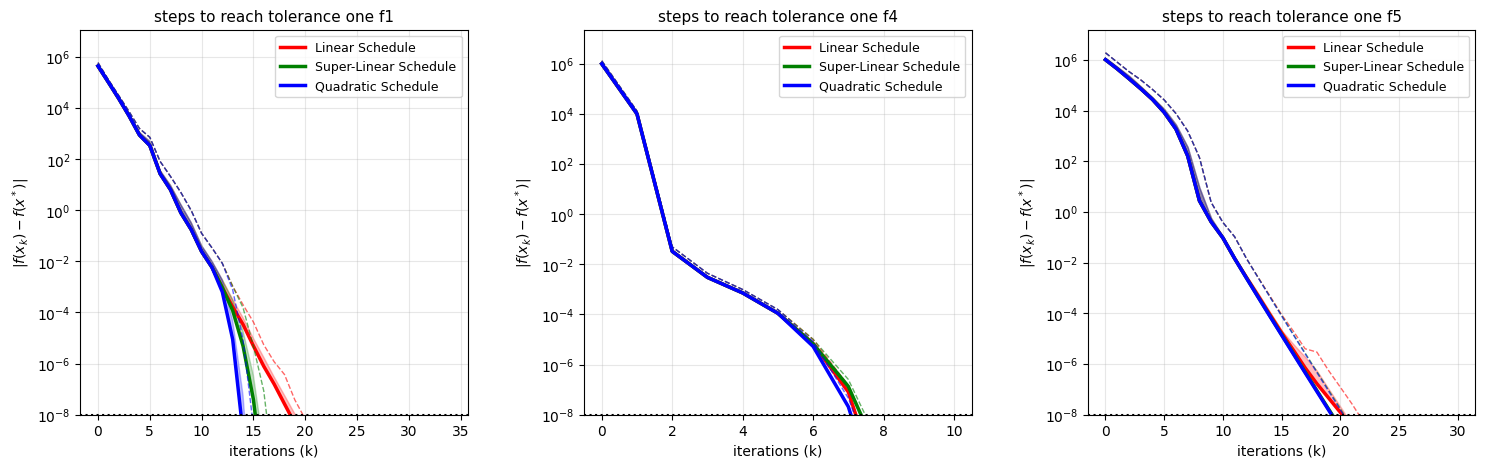
\includegraphics[width=0.9\textwidth]{billede2.png}
    \caption{Eta schedule comparison $d=20$, $\epsilon=1e-8$,$\rho=0.5$}
    \label{fig:schedules}
\end{figure}
We test a constant $\eta_k = 0.5$ (linear convergence), $\eta_k = \min\!\left(\frac{1}{2}, \|\nabla f(x_k)\|\right)$ (superlinear), and $\eta_k = \frac{1}{2}\min\!\left(\frac{1}{2}, \|\nabla f(x_k)\|\right)$ (superlinear, as used in Algorithm 6). We observe a difference in performance only on $f_1$. We attribute this to the fact that the theoretical rates derived in Lemma 4 are upper bounds on convergence, not exact descriptions.
\begin{equation}
    \|\nabla f(x_{k+1})\| \leq \frac{L}{2}\left(\frac{1}{\lambda_1(x_k)} + \lambda_N(x_k)\eta_k\right)^2 \|\nabla f(x_k)\|^2 + \eta_k\|\nabla f(x_k)\|,
\end{equation}
 On well-conditioned problems all three schedules converge rapidly in practice regardless of the theoretical distinction, because the quadratic term already dominates and the actual convergence rate is much better than the bound suggests.


\subsection{CG Steps During Optimization}

With a quadratic convergence schedule, the number of CG steps per outer 
iteration increases sharply as $\|\nabla f(x_k)\| \to 0$, since the inner 
stopping criterion $\varepsilon_k = \eta_k \|\nabla f(x_k)\|$ becomes 
increasingly stringent. By Theorem 6, CG requires at most $n$ steps to 
solve an $n$-dimensional system exactly, so the worst-case cost per Newton 
step grows linearly with dimension. This is observable in our experiments, 
where increasing the problem dimension leads to a rapid increase in total 
CG steps, underlining the computational advantage of using a looser 
schedule (linear or superlinear) in high-dimensional settings.



\begin{figure}[H]
    \centering
    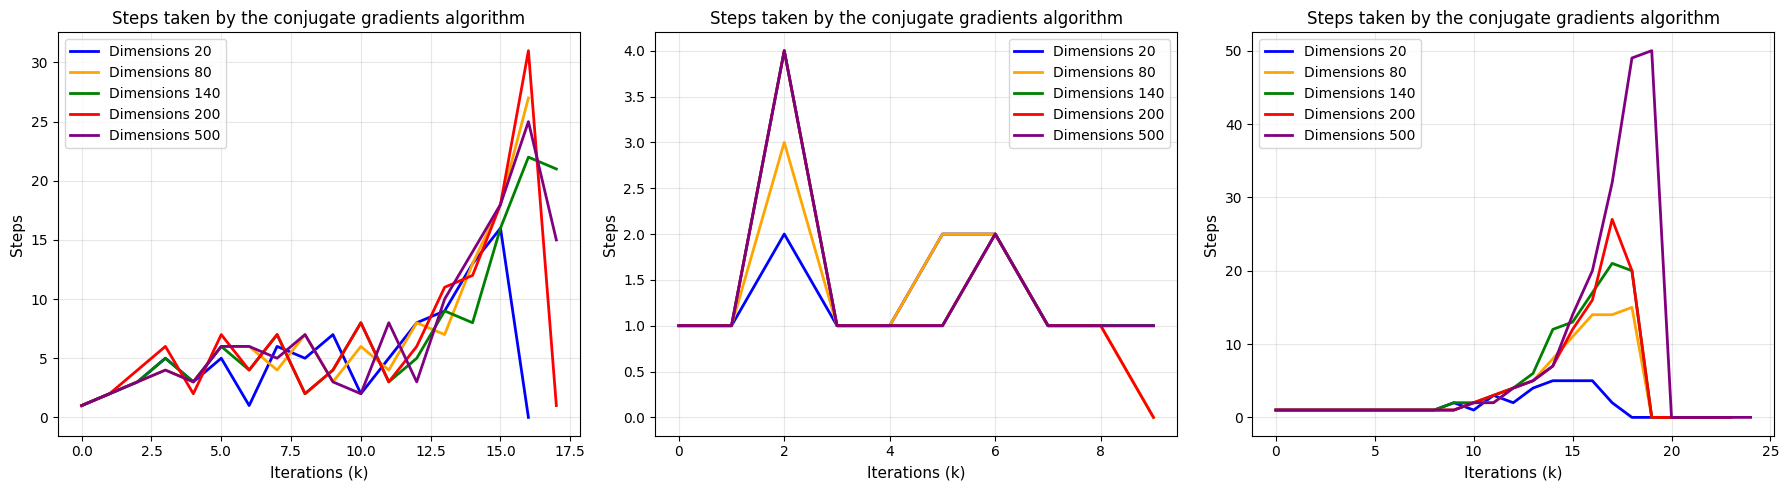
\includegraphics[width=0.9\textwidth]{billede3.png}
    \caption{CG steps comparison $\epsilon=1e-8$,$\rho=0.5$, $\eta_k = (SuperLinear)$}
    \label{fig:newtonsplot}
\end{figure}

\subsection{Comparison of Methods}

Figure~\ref{fig:comparison} compares Steepest Descent, Newton-BT and 
Inexact Newton. For $f_1$ and $f_4$, both Newton variants converge in very few iterations, clearly outperforming Steepest Descent. The Inexact Newton method closely 
matches exact Newton, showing that approximate inner solves preserve fast 
local convergence. For $f_5$, convergence slows near the optimum due to Hessian degeneracy, 
reducing the advantage of Newton-type methods.

\begin{figure}[H]
    \centering
    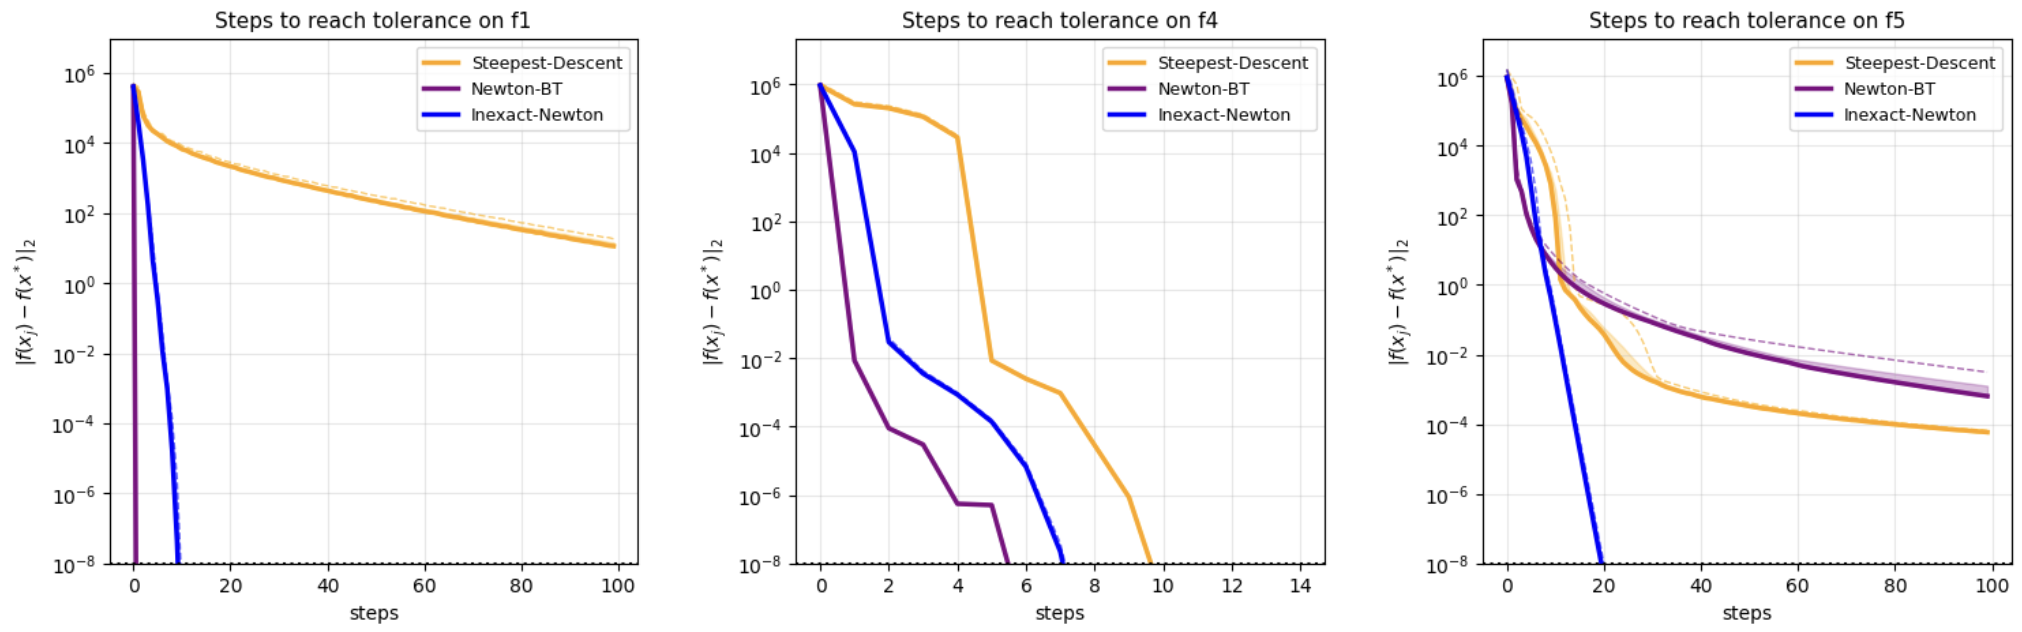
\includegraphics[width=0.9\textwidth]{billede.png}
    \caption{Newton's comparison $d=20$, $\epsilon=1e-8$,$\rho=0.5$, $\eta_k = (SuperLinear)$}
    \label{fig:comparison}
\end{figure}


\section{Conclusion}

Deriving equation (21) shows how gradient orthogonality makes the CG recurrence simpler. The approximate Newton method, solved via CG, achieves comparable performance to exact Newton while avoiding Hessian inversion. On well-conditioned functions ($f_1$, $f_4$), the method converges in few iterations regardless of the $\eta_k$ schedule, demonstrating the robustness of inexact Newton methods. The number of CG steps depends critically on function structure and proximity to the optimum, underscoring that computational efficiency is function-dependent rather than dimension-dependent alone.

\end{document}
